\documentclass[aspectratio=169, 12pt]{beamer}
\usepackage{fontspec}
\setmainfont{Arial}

\usetheme{Madrid}
\usecolortheme{default}

\usepackage{graphicx}
\usepackage{amsmath}
\usepackage{listings}
\usepackage{booktabs}
\usepackage{xcolor}
\usepackage{tabularx}
\usepackage{caption}

% Set code listing style
\lstset{
    basicstyle=\ttfamily\scriptsize,
    breaklines=true,
    keywordstyle=\color{blue},
    stringstyle=\color{red},
    commentstyle=\color{green!60!black},
    showstringspaces=false,
    frame=single,
    backgroundcolor=\color{gray!10}
}

\title[ML - Chap 05]{Chương 5: Máy học Véc-tơ Hỗ trợ (Support Vector Machines)}
\author[Giảng viên]{Giảng viên}
\institute[Đại học Đông Á]{Đại học Đông Á}
\date{\today}

\begin{document}

% 1
\begin{frame}
    \titlepage
\end{frame}

% 2
\begin{frame}{Mục tiêu của Chương}
    \begin{itemize}
        \item Hiểu khái niệm cốt lõi của \textbf{Support Vector Machines (SVM)}.
        \item Phân biệt giữa \textbf{Biên cứng (Hard Margin)} và \textbf{Biên mềm (Soft Margin)} trong phân loại SVM tuyến tính.
        \item Xử lý dữ liệu phi tuyến bằng kỹ thuật bổ sung đặc trưng hoặc \textbf{Kernel trick}.
        \item Áp dụng \textbf{Kernel Đa thức (Polynomial)} và \textbf{Kernel Gaussian RBF}.
        \item Khám phá cách sử dụng SVM cho bài toán \textbf{Hồi quy (Regression)}.
        \item Đi sâu vào \textbf{toán học phía sau SVM}: Bài toán tối ưu, Hàm mục tiêu và Đối ngẫu.
    \end{itemize}
\end{frame}

% 3
\begin{frame}{Mục lục}
    \tableofcontents
\end{frame}

%==================================================================
\section{1. Phân loại SVM Tuyến tính}
%==================================================================

% 4
\begin{frame}{1.1 Ý tưởng cơ bản của SVM}
    \begin{itemize}
        \item SVM là một trong những mô hình phổ biến và mạnh mẽ nhất trong Học máy truyền thống.
        \item SVM có thể giải quyết các bài toán phân loại tuyến tính, phi tuyến, và cả hồi quy.
        \item Tốt nhất cho các tập dữ liệu có kích thước \textbf{vừa và nhỏ} nhưng cực kỳ phức tạp.
        \item Ý tưởng chính: Tìm ra một \textbf{đường thẳng (hoặc siêu phẳng)} chia tách các lớp dữ liệu sao cho \textbf{khoảng cách} từ đường thẳng tới các điểm gần nhất của mỗi lớp là lớn nhất.
    \end{itemize}
\end{frame}

% 5
\begin{frame}{1.2 Mô hình Phân loại Biên Lớn (Large Margin Classification)}
    \begin{columns}
        \begin{column}{0.45\textwidth}
            \begin{itemize}
                \item Đường đứt nét ở giữa chia hai lớp một cách rõ ràng.
                \item Khoảng cách từ đường nét liền đến điểm dữ liệu gần nhất gọi là \textbf{Margin (Biên)}.
                \item SVM cố gắng làm cho lề này rộng nhất có thể.
                \item Các điểm nằm ngay trên rìa của lề được gọi là các \textbf{Véc-tơ Hỗ trợ (Support Vectors)}.
            \end{itemize}
        \end{column}
        \begin{column}{0.55\textwidth}
            \centering
            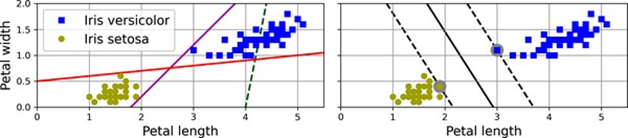
\includegraphics[width=\textwidth,height=0.65\textheight,keepaspectratio]{../machineLearningWeb/Figures/CH05/Hinh_5-1.png}
            \vspace{0.2cm}
            \textit{Hình 5-1: Ý tưởng Large Margin Classification}
        \end{column}
    \end{columns}
\end{frame}

% 6
\begin{frame}{1.3 Tính nhạy cảm với Tỉ lệ Đặc trưng (Feature Scaling)}
    \begin{columns}
        \begin{column}{0.4\textwidth}
            \begin{itemize}
                \item SVM rất nhạy cảm với tỉ lệ của các đặc trưng (thang đo).
                \item Nếu các đặc trưng có tỉ lệ quá chênh lệch (VD: x1 từ 0-1000, x2 từ 0-1), ranh giới quyết định sẽ gần như song song với trục lớn hơn.
                \item Do đó, luôn cần thực hiện \textbf{StandardScaler} trước khi đưa dữ liệu vào SVM.
            \end{itemize}
        \end{column}
        \begin{column}{0.6\textwidth}
            \centering
            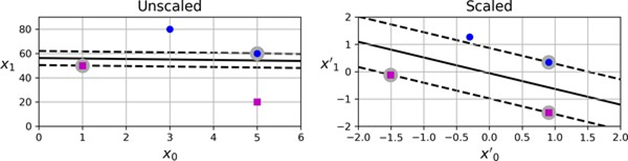
\includegraphics[width=\textwidth,height=0.65\textheight,keepaspectratio]{../machineLearningWeb/Figures/CH05/Hinh_5-2.png}
            \vspace{0.2cm}
            \textit{Hình 5-2: Sự khác biệt của lề khi chưa scale và đã scale}
        \end{column}
    \end{columns}
\end{frame}

% 7
\begin{frame}{1.4 Phân loại Biên Cứng (Hard Margin Classification)}
    \begin{itemize}
        \item Cố gắng chia tách tất cả các điểm một cách \textbf{hoàn hảo tuyệt đối}. Không điểm nào được phép nằm trong vùng lề hoặc nằm sai phía ranh giới.
        \item \textbf{Vấn đề 1:} Chỉ hoạt động được khi dữ liệu phân tách tuyến tính (Linearly Separable).
        \item \textbf{Vấn đề 2:} Rất nhạy cảm với Điểm bất thường (Outliers). Một nhiễu nhỏ cũng có thể làm biến dạng ranh giới.
    \end{itemize}
\end{frame}

% 8
\begin{frame}{1.5 Tác động của Điểm bất thường (Outliers)}
    \begin{columns}
        \begin{column}{0.5\textwidth}
            \centering
            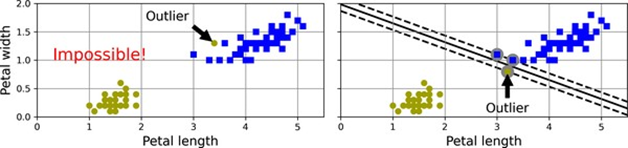
\includegraphics[width=\textwidth,height=0.6\textheight,keepaspectratio]{../machineLearningWeb/Figures/CH05/Hinh_5-3.png}
            \vspace{0.2cm}
            \textit{Hình 5-3: Biên Cứng bị bóp méo hoặc thất bại khi có outlier}
        \end{column}
        \begin{column}{0.5\textwidth}
            \begin{itemize}
                \item Hình bên trái: Một điểm xanh rơi vào vùng lớp đỏ khiến thuật toán không thể vẽ được đường thẳng chia cách hoàn hảo.
                \item Hình bên phải: Một outlier làm lề bị co hẹp lại một cách cực đoan, mô hình mất tính tổng quát.
            \end{itemize}
        \end{column}
    \end{columns}
\end{frame}

% 9
\begin{frame}{1.6 Phân loại Biên Mềm (Soft Margin Classification)}
    \begin{itemize}
        \item Để tránh những vấn đề của Biên cứng, ta sử dụng một mô hình linh hoạt hơn.
        \item Mục tiêu mới: Tìm sự cân bằng giữa việc \textbf{giữ cho lề rộng nhất có thể} và \textbf{hạn chế tối đa các điểm vi phạm lề} (Margin Violations).
        \item Đây gọi là Phân loại Biên mềm (Soft Margin Classification).
    \end{itemize}
\end{frame}

% 10
\begin{frame}{1.7 Siêu tham số C trong Scikit-Learn}
    \begin{columns}
        \begin{column}{0.4\textwidth}
            \begin{itemize}
                \item Tham số `C` điều khiển sự cân bằng trong Biên mềm.
                \item \textbf{C nhỏ:} Lề rộng hơn, nhưng cho phép nhiều điểm vi phạm lề (Tăng bias, Giảm variance). Dễ bị Underfitting.
                \item \textbf{C lớn:} Lề hẹp lại để hạn chế vi phạm lề (Giảm bias, Tăng variance). Dễ bị Overfitting.
            \end{itemize}
        \end{column}
        \begin{column}{0.6\textwidth}
            \centering
            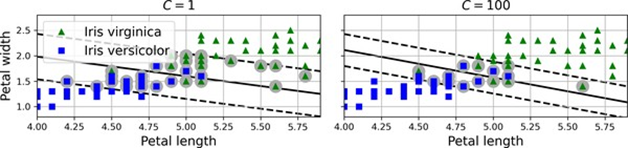
\includegraphics[width=\textwidth,height=0.65\textheight,keepaspectratio]{../machineLearningWeb/Figures/CH05/Hinh_5-4.png}
            \vspace{0.2cm}
            \textit{Hình 5-4: So sánh khi C thấp (trái) và C cao (phải)}
        \end{column}
    \end{columns}
\end{frame}

% 11
\begin{frame}[fragile]{1.8 Triển khai LinearSVM bằng Python}
\begin{lstlisting}[language=Python]
import numpy as np
from sklearn import datasets
from sklearn.pipeline import Pipeline
from sklearn.preprocessing import StandardScaler
from sklearn.svm import LinearSVC

# Tai du lieu Iris (Hoa diem vi)
iris = datasets.load_iris()
X = iris["data"][:, (2, 3)]  # Chieu dai, chieu rong canh hoa
y = (iris["target"] == 2).astype(np.float64)  # Iris virginica

# Xay dung Pipeline: chuan hoa + huan luyen
svm_clf = Pipeline([
    ("scaler", StandardScaler()),
    ("linear_svc", LinearSVC(C=1, loss="hinge", random_state=42))
])

svm_clf.fit(X, y)
print("Du doan:", svm_clf.predict([[5.5, 1.7]])) # Output: [1.]
\end{lstlisting}
\end{frame}


%==================================================================
\section{2. Phân loại SVM Phi tuyến}
%==================================================================

% 12
\begin{frame}{2.1 Giới thiệu SVM Phi tuyến}
    \begin{itemize}
        \item Rất nhiều bộ dữ liệu thực tế không thể phân tách bằng một đường thẳng.
        \item Một phương pháp đơn giản để xử lý tập dữ liệu phi tuyến là \textbf{thêm nhiều đặc trưng (Features) mới}, chẳng hạn như đặc trưng đa thức (Polynomial).
        \item Dữ liệu gốc ở 1D có thể không tách được, nhưng khi chiếu lên không gian 2D, ta có thể dùng đường thẳng để tách!
    \end{itemize}
\end{frame}

% 13
\begin{frame}{2.2 Minh họa Thêm đặc trưng đa thức}
    \begin{columns}
        \begin{column}{0.4\textwidth}
            \begin{itemize}
                \item Hình bên trái: Các điểm đỏ và xanh trên một trục 1D ($x_1$). Rõ ràng không có 1 điểm cắt nào phân chia hoàn hảo.
                \item Khi ta thêm đặc trưng mới $x_2 = (x_1)^2$.
                \item Hình bên phải: Trong không gian 2D ($x_1, x_2$), dữ liệu đã trở nên \textbf{phân tách tuyến tính}.
            \end{itemize}
        \end{column}
        \begin{column}{0.6\textwidth}
            \centering
            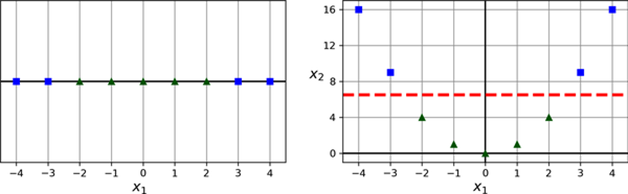
\includegraphics[width=\textwidth,height=0.6\textheight,keepaspectratio]{../machineLearningWeb/Figures/CH05/Hinh_5-5.png}
            \vspace{0.2cm}
            \textit{Hình 5-5: Thêm đặc trưng $x_2 = x_1^2$ giúp phân tách tuyến tính}
        \end{column}
    \end{columns}
\end{frame}

% 14
\begin{frame}{2.3 Phân tách Dataset "Moons" (Hai nửa vành trăng)}
    \begin{columns}
        \begin{column}{0.4\textwidth}
            \begin{itemize}
                \item Bộ dữ liệu *Make Moons* gồm 2 nửa vành khuyên lồng vào nhau.
                \item Sử dụng `PolynomialFeatures` kết hợp `StandardScaler` và `LinearSVC`.
                \item Đường cong ranh giới quyết định rất linh hoạt và phân loại chính xác các điểm.
            \end{itemize}
        \end{column}
        \begin{column}{0.6\textwidth}
            \centering
            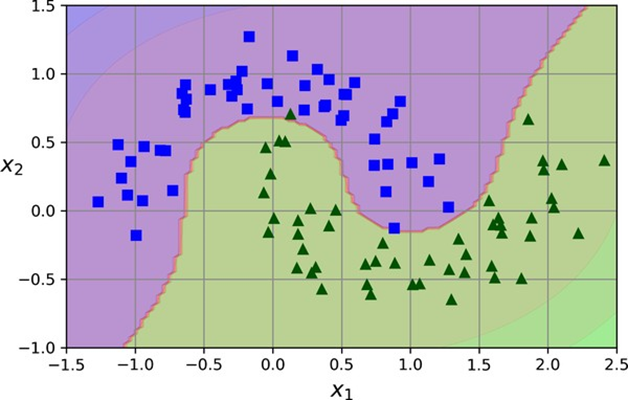
\includegraphics[width=\textwidth,height=0.65\textheight,keepaspectratio]{../machineLearningWeb/Figures/CH05/Hinh_5-6.png}
            \vspace{0.2cm}
            \textit{Hình 5-6: Ranh giới quyết định của Linear SVM với Polynomial Features}
        \end{column}
    \end{columns}
\end{frame}

% 15
\begin{frame}{2.4 Kernel Trick (Thủ thuật Kernel)}
    \begin{itemize}
        \item Việc tạo ra đặc trưng đa thức có bậc cao (Degree = 10, 20) sẽ tạo ra vô số các đặc trưng mới, làm chậm mô hình (Khủng hoảng chiều không gian - Curse of Dimensionality).
        \item May mắn thay, với SVM ta có một phép màu toán học gọi là \textbf{Kernel trick}.
        \item \textbf{Kernel Trick} cho phép SVM tính toán ra kết quả phân loại giống y hệt như việc ta thêm hàng tỉ đặc trưng đa thức, nhưng thực tế \textbf{nó không hề thêm một đặc trưng nào}. Do đó, không làm chậm thuật toán!
    \end{itemize}
\end{frame}

% 16
\begin{frame}{2.5 Kernel Đa thức (Polynomial Kernel)}
    \begin{columns}
        \begin{column}{0.45\textwidth}
            \begin{itemize}
                \item `SVC(kernel="poly", degree=3)`
                \item Tham số `coef0`: Kiểm soát mức độ ảnh hưởng của đa thức bậc cao so với đa thức bậc thấp.
                \item Hình ảnh cho thấy sự khác biệt giữa mô hình bậc 3 (trái) và bậc 10 (phải).
            \end{itemize}
        \end{column}
        \begin{column}{0.55\textwidth}
            \centering
            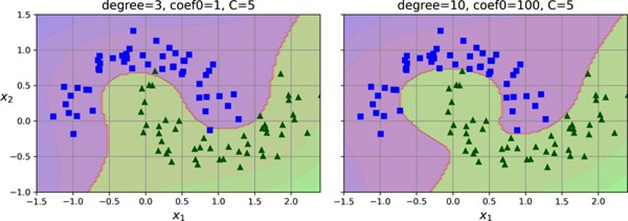
\includegraphics[width=\textwidth,height=0.65\textheight,keepaspectratio]{../machineLearningWeb/Figures/CH05/Hinh_5-7.png}
            \vspace{0.2cm}
            \textit{Hình 5-7: Polynomial Kernel với bậc 3 và 10}
        \end{column}
    \end{columns}
\end{frame}

% 17
\begin{frame}{2.6 Đặc trưng tương tự (Similarity Features)}
    \begin{itemize}
        \item Một kỹ thuật khác: Bổ sung các đặc trưng sử dụng \textbf{Hàm tương tự (Similarity Function)}, đo lường mỗi mẫu giống các Mốc (Landmarks) đến mức nào.
        \item Ví dụ: Gaussian Radial Basis Function (RBF).
        \item Công thức: $\phi_{\gamma}(x, \ell) = \exp(-\gamma ||x - \ell||^2)$
        \item Giá trị này dạng hình chuông, thay đổi từ 0 (rất xa) đến 1 (ngay tại mốc).
    \end{itemize}
\end{frame}

% 18
\begin{frame}{2.7 Minh họa Hàm Gaussian RBF}
    \begin{columns}
        \begin{column}{0.4\textwidth}
            \begin{itemize}
                \item Đặt mốc tại $x_1=-2$ và $x_1=1$.
                \item Chuyển điểm $x=-1$ thành 2 chiều mới: khoảng cách tới mốc 1 và khoảng cách tới mốc 2.
                \item Giờ đây tập dữ liệu đã có thể phân tách tuyến tính bằng 1 đường thẳng.
            \end{itemize}
        \end{column}
        \begin{column}{0.6\textwidth}
            \centering
            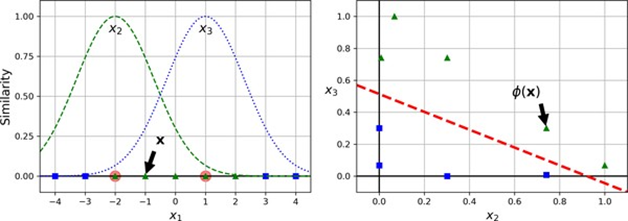
\includegraphics[width=\textwidth,height=0.65\textheight,keepaspectratio]{../machineLearningWeb/Figures/CH05/Hinh_5-8.png}
            \vspace{0.2cm}
            \textit{Hình 5-8: Sử dụng Similarity Features phân tách dữ liệu 1D}
        \end{column}
    \end{columns}
\end{frame}

% 19
\begin{frame}{2.8 Gaussian RBF Kernel}
    \begin{columns}
        \begin{column}{0.4\textwidth}
            \begin{itemize}
                \item Giống đa thức, ta dùng \textbf{Kernel RBF} để hưởng lợi ích của vô vàn các Mốc (Landmarks) mà không phải tính toán chi phí cao.
                \item `SVC(kernel="rbf", gamma=5, C=0.001)`
                \item Tham số `gamma` ($\gamma$): Định hình độ hẹp/rộng của quả chuông.
            \end{itemize}
        \end{column}
        \begin{column}{0.6\textwidth}
            \centering
            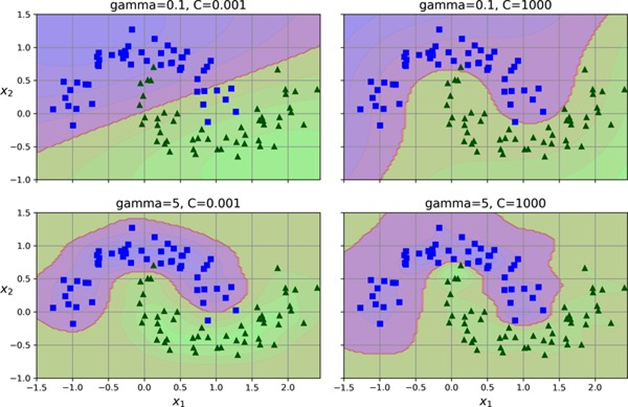
\includegraphics[width=\textwidth,height=0.65\textheight,keepaspectratio]{../machineLearningWeb/Figures/CH05/Hinh_5-9.png}
            \vspace{0.2cm}
            \textit{Hình 5-9: Hiệu ứng của $\gamma$ và $C$ lên SVM Kernel RBF}
        \end{column}
    \end{columns}
\end{frame}

% 20
\begin{frame}{2.9 Điều chỉnh siêu tham số Gamma và C}
    \begin{itemize}
        \item \textbf{Gamma ($\gamma$) lớn:} Quả chuông nhọn hẹp. Ranh giới uốn lượn sát theo từng điểm dữ liệu (Overfitting).
        \item \textbf{Gamma ($\gamma$) nhỏ:} Quả chuông rộng, mượt. Ranh giới mượt mà hơn (Underfitting).
        \item Lời khuyên: Nếu mô hình bị Overfitting, hãy giảm $\gamma$. Ngược lại, hãy tăng $\gamma$. (Tương tự như C).
        \item Rule of thumb: Khi nghi ngờ, hãy luôn thử \textbf{Linear Kernel} trước, sau đó tới \textbf{Gaussian RBF Kernel}.
    \end{itemize}
\end{frame}


%==================================================================
\section{3. Lớp SVM \& Hồi quy SVM}
%==================================================================

% 21
\begin{frame}{3.1 Các Lớp của Scikit-Learn cho SVM}
    \begin{itemize}
        \item `LinearSVC`: Dùng thư viện LIBLINEAR, tối ưu cho tập dữ liệu cực lớn, phức tạp thời gian $\mathcal{O}(m \times n)$. (Chỉ chạy tuyến tính).
        \item `SVC`: Dùng thư viện LIBSVM, hỗ trợ Kernel trick. Phức tạp thời gian $\mathcal{O}(m^2 \times n)$ đến $\mathcal{O}(m^3 \times n)$. (Quá chậm nếu số lượng mẫu > 100,000).
        \item `SGDClassifier(loss="hinge")`: Huấn luyện Gradient Descent ngẫu nhiên, hữu ích cho tập dữ liệu khổng lồ (Out-of-core learning).
    \end{itemize}
\end{frame}

% 22
\begin{frame}{3.2 Ý tưởng Hồi quy bằng SVM}
    \begin{itemize}
        \item Thuật toán SVM cực kỳ đa năng. Nó không chỉ phân loại tốt mà còn hồi quy (Dự đoán giá trị số liên tục) xuất sắc!
        \item Trong \textbf{Phân loại SVM}, mục tiêu là để dải lề rộng nhất nhưng KHÔNG chứa bất cứ điểm vi phạm nào bên trong dải lề.
        \item Ngược lại, trong \textbf{Hồi quy SVM}, mục tiêu là đưa CÀNG NHIỀU ĐIỂM VÀO BÊN TRONG dải lề càng tốt, trong khi hạn chế số điểm rơi ra ngoài dải lề.
        \item Độ rộng lề được kiểm soát bởi siêu tham số Epsilon ($\epsilon$).
    \end{itemize}
\end{frame}

% 23
\begin{frame}{3.3 Minh họa SVM Regression Tuyến tính}
    \begin{columns}
        \begin{column}{0.4\textwidth}
            \begin{itemize}
                \item Hình bên minh họa `LinearSVR`.
                \item Việc thêm nhiều điểm dữ liệu nằm bên trong biên không làm ảnh hưởng đến dự đoán của mô hình. 
                \item Mô hình gọi là \textbf{$\epsilon$-insensitive}.
                \item $\epsilon$ lớn (trái) lề rộng. $\epsilon$ nhỏ (phải) lề hẹp.
            \end{itemize}
        \end{column}
        \begin{column}{0.6\textwidth}
            \centering
            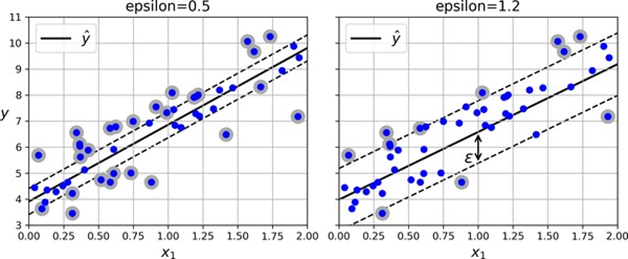
\includegraphics[width=\textwidth,height=0.65\textheight,keepaspectratio]{../machineLearningWeb/Figures/CH05/Hinh_5-10.png}
            \vspace{0.2cm}
            \textit{Hình 5-10: Hồi quy LinearSVR với các giá trị $\epsilon$ khác nhau}
        \end{column}
    \end{columns}
\end{frame}

% 24
\begin{frame}{3.4 Hồi quy SVM Phi tuyến (Nonlinear SVR)}
    \begin{columns}
        \begin{column}{0.45\textwidth}
            \begin{itemize}
                \item Hồi quy SVM cũng hỗ trợ Kernel trick thông qua lớp `SVR(kernel="poly")`.
                \item Trong hình là dữ liệu theo dạng hàm bậc 2. Mô hình có thể bám rất sát xu hướng với đường cong mịn màng.
                \item C nhỏ (trái): Mô hình tự do, linh hoạt.
                \item C lớn (phải): Ít sai số, sát dữ liệu hơn (ít regularization).
            \end{itemize}
        \end{column}
        \begin{column}{0.55\textwidth}
            \centering
            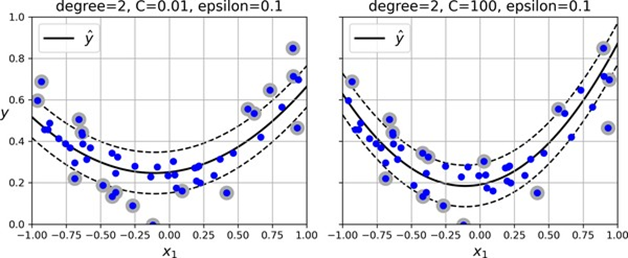
\includegraphics[width=\textwidth,height=0.6\textheight,keepaspectratio]{../machineLearningWeb/Figures/CH05/Hinh_5-11.png}
            \vspace{0.2cm}
            \textit{Hình 5-11: Hồi quy SVM phi tuyến bằng Kernel Đa thức}
        \end{column}
    \end{columns}
\end{frame}


%==================================================================
\section{4. Toán học: Bên trong Thuật toán SVM}
%==================================================================

% 25
\begin{frame}{4.1 Hàm Quyết định (Decision Function)}
    \begin{itemize}
        \item SVM tuyến tính dự đoán bằng cách tính hàm quyết định (Decision Function):
        \item Hàm số: $f(\mathbf{x}) = \mathbf{w}^T \cdot \mathbf{x} + b = w_1 x_1 + \cdots + w_n x_n + b$
        \item Nếu kết quả dương, dự đoán lớp $1$ (Tích cực). Nếu âm, dự đoán lớp $0$ (Tiêu cực).
        \item $\hat{y} = 1$ if $\mathbf{w}^T \mathbf{x} + b \ge 0$, else $0$.
    \end{itemize}
\end{frame}

% 26
\begin{frame}{4.2 Đồ thị Không gian Hàm quyết định}
    \begin{columns}
        \begin{column}{0.4\textwidth}
            \begin{itemize}
                \item Không gian 3 chiều: Trục Z là giá trị của hàm quyết định.
                \item Mặt phẳng cắt tại $Z=0$ tạo thành ranh giới quyết định (Đường liền đen).
                \item Đường lề đứt nét tương ứng với mặt cắt $Z=1$ và $Z=-1$.
            \end{itemize}
        \end{column}
        \begin{column}{0.6\textwidth}
            \centering
            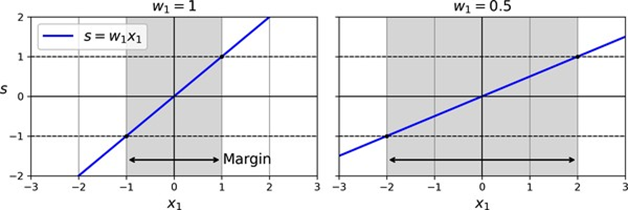
\includegraphics[width=\textwidth,height=0.65\textheight,keepaspectratio]{../machineLearningWeb/Figures/CH05/Hinh_5-12.png}
            \vspace{0.2cm}
            \textit{Hình 5-12: Decision function cho mô hình Iris Dataset 2D}
        \end{column}
    \end{columns}
\end{frame}

% 27
\begin{frame}{4.3 Mối liên hệ giữa Vector Trọng số (w) và Biên}
    \begin{columns}
        \begin{column}{0.4\textwidth}
            \begin{itemize}
                \item Kích thước của véc-tơ trọng số $\mathbf{w}$ xác định độ dốc của mặt phẳng hàm.
                \item Nếu chia đôi độ dốc $\mathbf{w}$, độ rộng của lề (Margin) sẽ nhân đôi!
                \item Để có Margin cực đại, ta phải \textbf{tối thiểu hóa độ lớn của $\mathbf{w}$}, tức là $||\mathbf{w}||$.
            \end{itemize}
        \end{column}
        \begin{column}{0.6\textwidth}
            \centering
            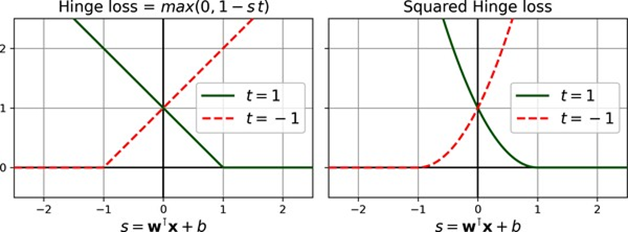
\includegraphics[width=\textwidth,height=0.65\textheight,keepaspectratio]{../machineLearningWeb/Figures/CH05/Hinh_5-13.png}
            \vspace{0.2cm}
            \textit{Hình 5-13: Trọng số $\mathbf{w}$ càng nhỏ, Lề margin càng lớn}
        \end{column}
    \end{columns}
\end{frame}

% 28
\begin{frame}{4.4 Hàm Mục Tiêu của Phân loại Biên Cứng}
    \begin{itemize}
        \item Ta muốn tối thiểu hóa $||\mathbf{w}||$ (để lề rộng nhất).
        \item Điều kiện ràng buộc: Tất cả mẫu lớp 1 phải có $f(\mathbf{x}) \ge 1$, và lớp 0 phải có $f(\mathbf{x}) \le -1$.
        \item Đặt $t^{(i)} = 1$ nếu $y^{(i)}=1$ và $t^{(i)} = -1$ nếu $y^{(i)}=0$. Ràng buộc gộp lại thành: $t^{(i)}(\mathbf{w}^T \mathbf{x}^{(i)} + b) \ge 1$ với mọi mẫu.
        \item Bài toán tối ưu hóa có ràng buộc:
        \item Cực tiểu hóa: $\frac{1}{2} \mathbf{w}^T \mathbf{w}$
        \item Sao cho: $t^{(i)}(\mathbf{w}^T \mathbf{x}^{(i)} + b) \ge 1$ $\forall i$
    \end{itemize}
\end{frame}

% 29
\begin{frame}{4.5 Hàm Mục Tiêu của Phân loại Biên Mềm}
    \begin{itemize}
        \item Trong Biên mềm, ta chấp nhận lỗi. Ta định nghĩa biến Slack $\zeta^{(i)} \ge 0$.
        \item $\zeta^{(i)}$ đo lường mức độ mẫu thứ $i$ được phép vi phạm lề.
        \item Tối thiểu hóa 2 mục tiêu mâu thuẫn nhau: làm cho $\mathbf{w}$ nhỏ nhất và làm cho tổng $\zeta$ nhỏ nhất.
        \item Bài toán tối ưu: Cực tiểu hóa $\frac{1}{2} \mathbf{w}^T \mathbf{w} + C \sum_{i=1}^m \zeta^{(i)}$
        \item Siêu tham số $C$ xác định sự đánh đổi giữa hai mục tiêu này.
    \end{itemize}
\end{frame}

% 30
\begin{frame}{4.6 Trình giải Bài toán (Solvers)}
    \begin{itemize}
        \item Đây là các bài toán \textbf{Quy hoạch Toàn phương (Quadratic Programming - QP)} có lời giải tối ưu toàn cục.
        \item Có rất nhiều solver có sẵn để giải: SMO, LIBLINEAR, LIBSVM.
        \item Có một dạng khác: Dùng Gradient Descent thông thường để cực tiểu hóa Hinge Loss. Đó chính là `SGDClassifier`.
    \end{itemize}
\end{frame}

% 31
\begin{frame}{4.7 Hinge Loss}
    \begin{itemize}
        \item Hàm mất mát Hinge: $\max(0, 1 - t)$
        \item Nó bằng 0 nếu $t \ge 1$ (điểm đã qua khỏi dải lề và nằm đúng phần).
        \item Nó tăng tuyến tính khi $t < 1$. Điều này tạo ra hình dạng cái bản lề.
        \item Hàm này không có đạo hàm tại $t=1$, nhưng vẫn dùng Subgradient để tối ưu bằng SGD được.
    \end{itemize}
\end{frame}

% 32
\begin{frame}{4.8 Bài toán Đối ngẫu (Dual Problem)}
    \begin{itemize}
        \item Bất kỳ bài toán Tối ưu hóa có ràng buộc (Primal Problem) nào cũng có một bài toán song sinh đi kèm gọi là bài toán Đối ngẫu (Dual Problem).
        \item Thường thì giải Dual dễ hơn Primal trong SVM khi số lượng quan sát m bé hơn số lượng đặc trưng n.
        \item Quan trọng hơn: Nhờ dạng Đối ngẫu mà phép màu \textbf{Kernel trick} mới có thể thực hiện được, điều mà dạng Primal không làm được.
    \end{itemize}
\end{frame}

% 33
\begin{frame}{4.9 Đẳng thức Kernel (Mercer's Theorem)}
    \begin{itemize}
        \item Thay vì ánh xạ điểm $x$ qua $\phi(x)$ (hàm biến đổi đa thức khổng lồ), ta chỉ cần tìm ra một hàm $K(\mathbf{a}, \mathbf{b})$.
        \item Hàm Kernel $K$ tính ra \textbf{tích vô hướng} của $\phi(\mathbf{a})^T \phi(\mathbf{b})$ cực kì nhanh gọn.
        \item Các Kernel phổ biến:
        \begin{itemize}
            \item Tuyến tính: $K(\mathbf{a}, \mathbf{b}) = \mathbf{a}^T \mathbf{b}$
            \item Đa thức: $K(\mathbf{a}, \mathbf{b}) = (\gamma \mathbf{a}^T \mathbf{b} + r)^d$
            \item Gaussian RBF: $K(\mathbf{a}, \mathbf{b}) = \exp(-\gamma ||\mathbf{a} - \mathbf{b}||^2)$
            \item Sigmoid: $K(\mathbf{a}, \mathbf{b}) = \tanh(\gamma \mathbf{a}^T \mathbf{b} + r)$
        \end{itemize}
    \end{itemize}
\end{frame}


%==================================================================
\section{5. Tổng kết chương}
%==================================================================

% 34
\begin{frame}{5.1 Ôn tập: Kiến trúc của SVM}
    \begin{itemize}
        \item SVM là một mô hình phân loại dựa trên khoảng cách (Lề phân cách).
        \item Có hai biến thể là Tuyến tính (Dùng Hinge Loss, Solver cực nhanh) và Phi tuyến tính (Dùng Kernel).
        \item Lề cứng nghiêm ngặt tuyệt đối, lề mềm dùng tham số C để cân bằng lỗi.
        \item Các bài toán được mô hình hóa chặt chẽ dựa trên Quy hoạch Toàn phương.
    \end{itemize}
\end{frame}

% 35
\begin{frame}{5.2 Ứng dụng phổ biến của SVM}
    \begin{itemize}
        \item Phân loại văn bản và phân tích cú pháp (Text/Categorization)
        \item Nhận dạng hình ảnh (Image recognition, MNIST)
        \item Phân loại gen tin sinh học (Bioinformatics, ung thư, protein)
        \item Hồi quy dự đoán tài chính.
    \end{itemize}
\end{frame}

% 36
\begin{frame}{5.3 Ưu điểm của SVM}
    \begin{itemize}
        \item Hiệu quả với dữ liệu có chiều cao (Số lượng Đặc trưng lớn).
        \item Vẫn tối ưu cực tốt khi Không gian chiều dữ liệu lớn hơn cả số mẫu ($n > m$).
        \item Tiết kiệm bộ nhớ vì hàm ra quyết định chỉ phụ thuộc một nhóm các Support Vectors.
        \item Có nền tảng lý thuyết tối ưu lồi (Convex Optimization) bảo đảm hội tụ tới Tối ưu Toàn cục (Global Optimum), không bị dính vào tối ưu cục bộ như Neural Networks.
    \end{itemize}
\end{frame}

% 37
\begin{frame}{5.4 Nhược điểm của SVM}
    \begin{itemize}
        \item Thời gian huấn luyện (O(n$^2$) đến O(n$^3$)) rất chậm nếu bộ dữ liệu có trên 100,000 dòng.
        \item Không thể cho ra Xác suất (Probability) một cách tự nhiên như Logistic Regression (Phải dùng Platt Scaling tốn kém).
        \item Cực kỳ nhạy cảm và bắt buộc phải có bước chuẩn hóa (Scale) dữ liệu.
        \item Không diễn giải dễ dàng (Black-box model).
    \end{itemize}
\end{frame}

% 38
\begin{frame}{5.5 Bài tập Thực hành: Phân loại Ảnh Chữ Số}
    \begin{itemize}
        \item Đề bài: Xây dựng bộ phân loại SVM trên bộ dữ liệu MNIST.
        \item MNIST gồm các ảnh xám 28x28 pixel của các chữ số viết tay từ 0-9.
        \item Vì SVM mặc định là nhị phân (Binary), nó sẽ sử dụng chiến lược One-versus-Rest (OvR) hoặc One-versus-One (OvO) tự động bên dưới Scikit-Learn.
    \end{itemize}
\end{frame}

% 39
\begin{frame}[fragile]{5.6 Code Gợi ý Huấn luyện MNIST bằng SVM}
\begin{lstlisting}[language=Python]
from sklearn.datasets import fetch_openml
from sklearn.svm import SVC
from sklearn.metrics import accuracy_score

# 1. Tai du lieu va Scale (0-255 -> 0-1)
mnist = fetch_openml('mnist_784', version=1)
X, y = mnist["data"], mnist["target"]
X_train, X_test, y_train, y_test = X[:60000]/255., X[60000:]/255., y[:60000], y[60000:]

# 2. Xay dung mo hinh SVM voi RBF Kernel (Mac dinh)
svm_clf = SVC(gamma="scale")
svm_clf.fit(X_train[:10000], y_train[:10000]) # Huan luyen tap nho cho nhanh

# 3. Kiem thu
y_pred = svm_clf.predict(X_test)
print("Accuracy:", accuracy_score(y_test, y_pred))
\end{lstlisting}
\end{frame}

% 40
\begin{frame}{5.7 Lựa chọn Mô hình phù hợp}
    \begin{itemize}
        \item Đừng lao vào Deep Learning ngay khi làm dự án thực tế.
        \item Luôn thử Logistic Regression hoặc Random Forest trước làm Baseline.
        \item Sau đó thử SVM. Dù tốc độ đào tạo chậm, nhưng khả năng phân loại của SVM thường vượt trội với tập dữ liệu tabular (bảng).
    \end{itemize}
\end{frame}

% 41
\begin{frame}
    \centering
    \Huge \textbf{HỎI \& ĐÁP}
\end{frame}

\end{document}
